% Definiciones y constantes de estilo
% Clase del documento
\documentclass[a4paper,12pt,twoside,openright,titlepage]{book}

%
% Paquetes necesarios
%

% Símbolo del euro
\usepackage{eurosym}
% Codificación UTF8
\usepackage[utf8]{inputenc}
% Caracteres del español
\usepackage[spanish]{babel}
% Código, algoritmos, etc.
\usepackage{listings}
% Definición de colores
\usepackage{color}
% Extensión del paquete color
\usepackage[table,xcdraw]{xcolor}
% Márgenes
\usepackage{anysize}
% Cabecera y pie de página
\usepackage{fancyhdr}
% Estilo título capítulos
\usepackage{quotchap}
% Algoritmos (expresarlos mejor)
\usepackage{algorithmic}
% Citas mejoradas
\usepackage{cite}
% Títulos de secciones
\usepackage{titlesec}
% Fórmulas matemáticas
\usepackage[cmex10]{amsmath}
% Enumeraciones
\usepackage{enumerate}
% Páginas en blanco
\usepackage{emptypage}
% Separación entre cajas
\usepackage{float}
% Imágenes
\usepackage[pdftex]{graphicx}
% Mejora de las tablas
\usepackage{array}
% Mejora de los símbolos matemáticos
\usepackage{mdwmath}
% Separar figuras en subfiguras
\usepackage[caption=false,font=footnotesize]{subfig}
% Incluir pdfs externos
\usepackage{pdfpages}
% Mejoras sobre las cajas
\usepackage{fancybox}
% Apéndices
\usepackage{appendix}
% Marcadores (para el pdf)
\usepackage{bookmark}
% Estilo de enumeraciones
\usepackage{enumitem}
% Espacio entre líneas y párrafos
\usepackage{setspace}
% Glosario/Acrónimos
\usepackage[acronym]{glossaries}
% Fuentes
\usepackage[T1]{fontenc}

% Enlaces
\hypersetup{hidelinks,pageanchor=false,colorlinks,citecolor=Fuchsia,urlcolor=black,linkcolor=Cerulean}

% Fix warning
\setlength{\headheight}{16pt}

% Euro (€)
\DeclareUnicodeCharacter{20AC}{\euro}

% Estilo de la bibliografía
\bibliographystyle{IEEEtran}
\addto{\captionsspanish}{\renewcommand{\bibname}{Referencias}}

% Inclusión de gráficos
\graphicspath{{./graphics/}}

% Extensiones de gráficos
\DeclareGraphicsExtensions{.pdf,.jpeg,.jpg,.png}

% Definiciones de colores (para hidelinks)
\definecolor{LightCyan}{rgb}{0,0,0}
\definecolor{Cerulean}{rgb}{0,0,0}
\definecolor{Fuchsia}{rgb}{0,0,0}

% Keywords (español e inglés)
\def\keywordsEn{\vspace{.5em}
{\textbf{\textit{Key words ---}}\,\relax%
}}
\def\endkeywordsEn{\par}

\def\keywordsEs{\vspace{.5em}
{\textbf{\textit{Palabras clave ---}}\,\relax%
}}
\def\endkeywordsEs{\par}


% Abstract (español e inglés)
\def\abstractEs{\vspace{.5em}
{\textbf{\textit{Resumen ---}}\,\relax%
}}
\def\endabstractEs{\par}

\def\abstractEn{\vspace{.5em}
{\textbf{\textit{Abstract ---}}\,\relax%
}}
\def\endabstractEn{\par}

% Estilo páginas de capítulos
\fancypagestyle{plain}{
\fancyhf{}
\fancyfoot[CO]{\footnotesize\emph{\nombretrabajo}}
\fancyfoot[RO]{\thepage}
\renewcommand{\footrulewidth}{.6pt}
\renewcommand{\headrulewidth}{0.0pt}
}

% Estilo resto de páginas
\pagestyle{fancy}

% Estilo páginas impares
\fancyfoot[CO]{\footnotesize\emph{\nombretrabajo}}
\fancyfoot[RO]{\thepage}
\rhead[]{\leftmark}

% Estilo páginas pares
\fancyfoot[CE]{\emph{\pieparcen}}
\fancyfoot[LE]{\thepage}
\fancyfoot[RE]{\pieparizq}
\lhead[\leftmark]{}

% Guía del pie de página
\renewcommand{\footrulewidth}{.6pt}

% Nombre de los bloques de código
\renewcommand{\lstlistingname}{Código}

% Estilo de los lstlistings
\lstset{
    frame=tb,
    breaklines=true,
    postbreak=\raisebox{0ex}[0ex][0ex]{\ensuremath{\color{gray}\hookrightarrow\space}}
}

% Definiciones de funciones para los títulos
\newlength\salto
\setlength{\salto}{3.5ex plus 1ex minus .2ex}
\newlength\resalto
\setlength{\resalto}{2.3ex plus.2ex}

% Estilo de los acrónimos
\renewcommand{\acronymname}{Glosario}
\renewcommand{\glossaryname}{Glosario}
\pretolerance=2000
\tolerance=3000
\renewcommand{\glsnamefont}[1]{\makefirstuc{#1}}

% Pie de tabla
\addto\captionsspanish{
\def\tablename{Tabla}
\def\listtablename{\'Indice de tablas}
}

% Traducir appendix/appendices
\renewcommand\appendixtocname{Apéndices}
\renewcommand\appendixpagename{Apéndices}

% Comando code (lstlisting sin cambio de página)
\lstnewenvironment{code}[1][]%
  { \noindent\minipage{0.935\linewidth}\medskip
    \vspace{5mm}
    \lstset{basicstyle=\ttfamily\footnotesize,#1}}
  {\endminipage}

% Estilo JSON en listing
\colorlet{punct}{red!60!black}
\definecolor{background}{HTML}{EEEEEE}
\definecolor{delim}{RGB}{20,105,176}
\colorlet{numb}{magenta!60!black}
\lstdefinelanguage{json}{
    basicstyle=\normalfont\ttfamily,
    stepnumber=1,
    numbersep=8pt,
    showstringspaces=false,
    breaklines=true,
    backgroundcolor=\color{background},
    literate=
     *{0}{{{\color{numb}0}}}{1}
      {1}{{{\color{numb}1}}}{1}
      {2}{{{\color{numb}2}}}{1}
      {3}{{{\color{numb}3}}}{1}
      {4}{{{\color{numb}4}}}{1}
      {5}{{{\color{numb}5}}}{1}
      {6}{{{\color{numb}6}}}{1}
      {7}{{{\color{numb}7}}}{1}
      {8}{{{\color{numb}8}}}{1}
      {9}{{{\color{numb}9}}}{1}
      {:}{{{\color{punct}{:}}}}{1}
      {,}{{{\color{punct}{,}}}}{1}
      {\{}{{{\color{delim}{\{}}}}{1}
      {\}}{{{\color{delim}{\}}}}}{1}
      {[}{{{\color{delim}{[}}}}{1}
      {]}{{{\color{delim}{]}}}}{1},
}

% Definiciones de comandos
\newcommand{\nombreautor}{Juan Sidrach de Cardona Mora}
\newcommand{\nombretutor}{Dr. Sergio López-Buedo}
\newcommand{\nombretrabajo}{Interfaz web para la gestión de sondas de red de altas prestaciones}
\newcommand{\fecha}{Junio 2014}
\newcommand{\grado}{Doble Grado en Ingeniería Informática y Matemáticas}
\newcommand{\grupoInvestigacion}{High Performance Computing and Networking Research Group}
\newcommand{\departamento}{Dpto. de Tecnología Electrónica y de las Comunicaciones}
\newcommand{\facultad}{Escuela Politécnica Superior}
\newcommand{\universidad}{Universidad Autónoma de Madrid}
\newcommand{\pieparizq}{\href{https://github.com/JSidrach/NetWatcher}{\scriptsize{github.com/JSidrach/NetWatcher}}}
\newcommand{\pieparcen}{Trabajo de Fin de Grado}
\newcommand{\logoizq}{Logo_EPS}
\newcommand{\logoder}{Logo_UAM}
\newcommand{\correo}{juan.sidrach@gmail.com}

% Glosario y acrónimos
\makeglossaries
% Acrónimos

% TODO: Añadir aquí los acrónimos
% Ejemplo de acrónimo
\newacronym{FPGA}{FPGA}{Field-Programmable Gate Array}
\newacronym{IFG}{IFG}{InterFrame Gap (TODO)}

% Glosario

% TODO: Añadir aquí las definiciones del glosario
% Ejemplo de glosario
\newglossaryentry{bitstream}{name={bitstream},description={En este contexto se refiere al binario que configura el Hardware de la FPGA}}
\newglossaryentry{traza}{name={traza},plural={trazas},description={TODO: traza}}
\newglossaryentry{simple}{name={simple},description={TODO: simple}}
\newglossaryentry{pcap}{name={pcap},description={TODO: pcap}}


% Inicio del documento
\begin{document}

% Elección del idioma (español)
\selectlanguage{spanish}

%
% Portada
%
\pagenumbering{gobble}
\include{portada}
\hypersetup{pageanchor=true}

%
% Agradecimientos
%
\pagenumbering{Roman}
\setcounter{page}{0}
\include{src/agradecimientos}  

%
% Resumen
%
\include{src/resumen}

%
% Glosario
%
\printglossary[title=Glosario,toctitle=Glosario]
\printglossary[title=Acrónimos,toctitle=Acrónimos,type=\acronymtype]

%
% Tabla de contenidos
%
\tableofcontents
\listoftables
\listoffigures
\cleardoublepage

% Estilo de párrafo de los capítulos
\setlength{\parskip}{0.75em}
\renewcommand{\baselinestretch}{1.25}
% Interlineado
\spacing{1.3}
% Numeración contenido
\pagenumbering{arabic}
\setcounter{page}{1}

%
% Capítulos
%
\chapter{Introducción}

TODO: Introducción del trabajo
interfaz web para la gestión de sondas de red de altas prestaciones. HPCN. Ámbito, motivación y objetivos de este Trabajo de Fin de Grado, seguidos de una explicación sobre la estructura del documento.

Una sonda de red es simplemente un dispositivo capaz de capturar tráfico de red (sonda
pasiva) o de inyectarlo (sonda activa). Este dispositivo puede ser algo tan sencillo
como un ordenador convencional, en el que se ha instalado una tarjeta Ethernet
estándar o una tarjeta a medida basada en FPGA (ver la propuesta de proyecto
“Sistema basado en FPGA para la captura de tráfico en redes multigigabit Ethernet”).
Este ordenador típicamente correrá un sistema operativo Linux/GNU, y se habrán
instalado unos drivers especiales para poder acceder lo más eficientemente a la tarjeta
de red. Lo habitual es manejar la sonda desde línea de comandos. En este proyecto se
propone hacer una interfaz de usuario mucho más amigable, basada en web. En la
sonda correrá un servidor web, que mostrará una página con la que se podrá configurar
y manejar todos los aspectos de la sonda (capturar tráfico, reproducirlo, estado de la
sonda). Todas estas operaciones se corresponden con ejecutar programas de línea de
comandos, por lo que en resumidas cuentas este proyecto consiste en hacer un frontend
web para una interfaz de línea de comandos.
La interfaz web no solo tendrá una sección de controles para manejar la sonda, sino que
también mostrará su estado de una manera gráfica (medidores de nivel, etc.) y dibujará
alguna gráfica sencilla (bytes recibidos vs. tiempo, etc.)


\section{\'Ambito}

Trabajo de Fin de Grado

 sondas de red de altas prestaciones

grupo de investigación \textit{High Performance Computing and Networking}. 

TODO: Ámbito del trabajo


\section{Motivación}

Necesaria simplificación gestión de sondas de red de altas prestaciones por medio de una interfaz gráfica

ampliar la funcionalidad ofreciendo monitorización 
TODO: Motivación del trabajo


\section{Objetivos}

Este Trabajo de Fin de Grado tiene los siguientes objetivos principales:

\begin{itemize}
  \item Desarrollar una interfaz web que permita la gestión de sondas de red de altas prestaciones de manera intuitiva y sencilla.
  Desarrollar una interfaz web que permita la gestión de sondas de red de altas prestaciones de manera intuitiva y sencilla.
  Desarrollar una interfaz web que permita la gestión de sondas de red de altas prestaciones de manera intuitiva y sencilla.

  \item Monitorizar el estado del servidor al que está conectada una sonda de red de altas prestaciones.
Desarrollar una interfaz web que permita la gestión de sondas de red de altas prestaciones de manera intuitiva y sencilla.
Desarrollar una interfaz web que permita la gestión de sondas de red de altas prestaciones de manera intuitiva y sencilla.

  \item Registrar estadísticas sobre la utilización de las sondas de red de altas prestaciones.
Desarrollar una interfaz web que permita la gestión de sondas de red de altas prestaciones de manera intuitiva y sencilla.
Desarrollar una interfaz web que permita la gestión de sondas de red de altas prestaciones de manera intuitiva y sencilla.
\end{itemize}

\section{Estructura del documento}

En el capítulo \ref{cap:estadoDelArte} se realiza un análisis del estado del arte. Se analizan tanto los sistemas de captura y reproducción de tráfico web existentes como las interfaces de gestión y monitorización de estos sistemas, para posteriormente extraer conclusiones sobre lo estudiado.

En el capítulo \ref{cap:defProyecto} se define la aplicación que se va a diseñar, así como la metodología seguida y las herramientas utilizadas en el proyecto.
En el capítulo \ref{cap:requisitos} se describen los requisitos funcionales y no funcionales de la aplicación.

En el capítulo \ref{cap:disenho} se formaliza el diseño de la aplicación a implementar, comentando la arquitectura de la aplicación y los módulos en los que se divide.
En el capítulo \ref{cap:implementacion} se documenta la implementación de la aplicación, estructurada en dos partes bien diferenciadas: \gls{back-end} y \gls{front-end}.
En el capítulo \ref{cap:pruebas} se explica el proceso de pruebas seguido para la verificación y validación de la aplicación construida, comprobando así el correcto funcionamiento de la misma.
En el capítulo \ref{cap:mantenimiento} se espeficica cómo se va a realizar el mantenimiento de la aplicación.

En el capítulo \ref{cap:conclusiones} se exponen las conclusiones finales sobre el trabajo realizado. Por último, en el capítulo \ref{cap:lineasDeTrabajoFuturo} se plantean posibles líneas de trabajo futuro que podrían ser abordadas con el objetivo de mejorar y ampliar diferentes aspectos de la aplicación desarrollada.
\chapter{Estado del arte\label{cap:estadoDelArte}}

TODO: [Introducción]


\section{Sistemas de captura y/o reproducción de tráfico de red\label{sec:eda:sistemas_captura_reproducccion}}

TODO: Sistemas de captura y/o reproducción de tráfico de red

\section{FPGA HPCN\label{ssec:eda:fpga}}
TODO: Cambiar organización
Los posibles estados de la \gls{FPGA} son:
\begin{itemize}\label{fpga:estados}
  \item No programada
  \item Programada para reproducir
  \item Programada para capturar
  \item Montada para reproducir
  \item Montada para capturar
  \item Reproduciendo una \gls{traza}
  \item Capturando tráfico
\end{itemize}

\section{Sistemas de gestión y monitorización\label{sec:eda:sistemas_gestion_monitorizacion}}

TODO: Sistemas de gestión y monitorización


\section{Conclusiones\label{sec:eda:conclusiones}}

TODO: Conclusiones
\chapter{Definición del proyecto\label{cap:defProyecto}}

En este capítulo se definirán y explicarán el alcance del proyecto, la metodología de desarrollo escogida y las herramientas utilizadas.

\section{Alcance\label{sec:dp:alcance}}

Esta aplicación tiene como objetivo permitir mediante una interfaz web conocer el estado actual de una sonda de red, y gestionarla. Asímismo, se podrán manejar otros aspectos relacionados con la sonda, como el almacenamiento y manejo de las \glspl{traza} capturadas.

No se pretende sin embargo que la interfaz web sea capaz de interactuar con cualquier tipo de sonda de captura y reproducción de tráfico de red, sólo con la sonda seleccionada.
Tampoco entra dentro del alcance de este proyecto modificar el funcionamiento interno de la sonda, ni siquiera para mejorar sus prestaciones, ya que el objetivo final es simplemente facilitar la gestión de una sonda de red de altas prestacines y de otros componentes que intervienen en el sistema.

\section{Metodología\label{sec:dp:metodologia}}

\begin{figure}[!htp]
  \centering
  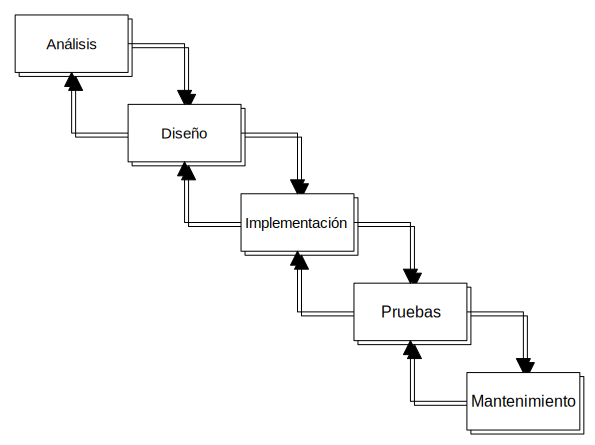
\includegraphics[width=0.7\textwidth,clip=true]{graphics/cascada_retroalimentacion}
  \caption{Modelo de ciclo de vida en cascada con retroalimentación.}
  \label{fig:cascada}
\end{figure}

Para el desarrollo de la aplicación se ha optado por seguir un ciclo de vida en cascada con retroalimentación (ver Figura \ref{fig:cascada}).
Este modelo ordena las etapas del proceso de desarrollo de software, de forma que sólo se pueda iniciar una fase cuando se ha finalizado la anterior.
Dada la naturaleza de este proyecto, era necesario periodo amplio de estudio del problema a resolver antes de poder codificar nada, siendo por ello este modelo más recomendable que adoptar alguna metodología ágil.
Por otra parte, se ha descartado utilizar un modelo iterativo o en espiral dado que conllevaría un mayor tiempo de desarrollo al tener que realizarse por módulos y de forma separada cada una de las fases definidas, en vez de simultáneamente y de forma global.
Además, el hecho de tener retroalimentación ha permitido volver a etapas anteriores en caso de que sea necesario para corregir algún aspecto del sistema.

La distribución temporal de las tareas y sus dependencias se resumen en el diagrama de Gantt de la Figura \ref{fig:gantt}.
A continuación se detallan la entradas, tareas y salidas de cada una de las fases del desarrollo del proyecto.

\begin{figure}[!htp]
  \centering
  \includegraphics[width=0.7\textwidth,clip=true]{graphics/gantt_white}
  \caption{Diagrama de Gantt de la planificación temporal del proyecto.}
  \label{fig:gantt}
\end{figure} 

\subsection*{Análisis\label{ssec:dp:analisis}}

Tareas
\begin{itemize}[leftmargin=3.5em]
  \item Analizar el estado del arte.
  \item Definir los objetivos de la aplicación.
  \item Especificar los requisitos funcionales y no funcionales.
\end{itemize}

Salida
\begin{itemize}[leftmargin=3.5em]
  \item Definición, objetivos y alcance del proyecto.
  \item Relación de requisitos.
\end{itemize}

\subsection*{Diseño y arquitectura\label{ssec:dp:disenho}}

Entrada
\begin{itemize}[leftmargin=3.5em]
  \item Relación de requisitos.
\end{itemize}

Tareas
\begin{itemize}[leftmargin=3.5em]
  \item Diseñar la arquitectura y módulos a implementar. 
  \item Diseñar la interfaz web.
\end{itemize}

Salida
\begin{itemize}[leftmargin=3.5em]
  \item Arquitectura de la aplicación.
  \item Diagramas de diseño.
  \item Maquetas de la interfaz web.
\end{itemize}

\subsection*{Implementación\label{ssec:dp:implementacion}}

Entrada
\begin{itemize}[leftmargin=3.5em]
  \item Información sobre la arquitectura y el diseño de la aplicación.
  \item Maquetas de la interfaz web.
\end{itemize}

Tareas
\begin{itemize}[leftmargin=3.5em]
  \item Codificar del \gls{back-end}.
  \item Codificar del \gls{front-end}.
\end{itemize}

Salida
\begin{itemize}[leftmargin=3.5em]
  \item Código de la aplicación.
  \item Documentación del código de la aplicación.
\end{itemize}

\subsection*{Pruebas\label{ssec:dp:pruebas}}

Entrada
\begin{itemize}[leftmargin=3.5em]
  \item Código de la aplicación.
\end{itemize}

Tareas
\begin{itemize}[leftmargin=3.5em]
  \item Realizar el plan de pruebas acordado.
  \item Evaluar el sistema final.
\end{itemize}

Salida
\begin{itemize}[leftmargin=3.5em]
  \item Código de la aplicación validado y verificado.
\end{itemize}

\subsection*{Mantenimiento\label{ssec:dp:mantenimiento}}

Entrada
\begin{itemize}[leftmargin=3.5em]
  \item Código de la aplicación validado y verificado.
\end{itemize}

Tareas
\begin{itemize}[leftmargin=3.5em]
  \item Analizar, implementar y probar las solicitudes de mejoras propuestas por usuarios. 
\end{itemize}

Salida
\begin{itemize}[leftmargin=3.5em]
  \item Código de la aplicación validado y verificado, con cambios menores propuestos por usuarios.
\end{itemize}


\section{Herramientas\label{sec:dp:herramientas}}

Para el desarrollo de este proyecto han sido necesarias herramientas que cubran las siguientes necesidades:

\begin{itemize}
  \item Control de versiones.
  \item Creación de diagramas y maquetas.
  \item Documentación de la aplicación.
  \item Plataforma base para el \gls{back-end}.
  \item Plataforma base para el \gls{front-end}.
\end{itemize}

A continuación se especifican las herramientas elegidas, exponiendo su utilidad.
Se detallan también las librerías externas de las que hace uso la aplicación.

\subsection*{Control de versiones: git\label{ssec:dp:git}}

En todo proyecto software es fundamental, especialmente si se alarga en el tiempo, hacer uso de una herramienta de control de versiones para el código y la documentación. Se ha elegido con este propósito utilizar la plataforma \textit{GitHub} \cite{github}, basada en \textit{git} \cite{git}, un sistema distribuido de control de versiones.
Esta plataforma es la más popular dentro de las herramientas de control de versiones, y tiene algunas ventajas importantes respecto a otros sistemas similares.

En primer lugar, ofrece alojamiento gratuito para proyectos de código abierto, y también para proyectos privados si se es estudiante. Gracias a esto se ha podido desarrollar todo el código de la aplicación en un proyecto privado, liberándolo al público al finalizar el desarrollo principal, de forma que cualquiera pueda utilizar y mejorar el código existente. 
Por otra parte, \textit{GitHub} añade a la funcionalidad de \textit{git} la posibilidad de crear una \textit{wiki} del proyecto de forma sencilla, característica que ha sido utilizada en el proyecto.
Finalmente, facilita la colaboración entre desarrolladores con una interfaz intuitiva y cuya curva de aprendizaje no es demasiado inclinada. 

\subsection*{Creación de diagramas y maquetas: Cacoo\label{ssec:dp:cacoo}}

Para el diseño de la aplicación se han realizado diagramas de flujo y de arquitectura del proyecto, así como maquetas de las diferentes pantallas de la interfaz web.
Para ello, se ha utilizado la herramienta \textit{Cacoo} \cite{cacoo}, ya que ofrece una licencia gratuita para estudiantes que permite exportar estos gráficos en formato vectorial \textit{svg}, que se pueden redimensionar sin pérdida de resolución.
Otra característica interesante es que está basada en tecnologías web, con lo que es accesible desde cualquier navegador, sin ser necesario instalar ningún programa adicional.

\subsection*{Documentación: phpDocumentor y apiDoc\label{ssec:dp:docs}}

Con el objetivo de documentar la aplicación, se buscó una librería que contase con características particulares.
Por un lado, que permitiese crear la documentación mediante anotaciones en el propio código, sin ralentizar demasiado la implementación del proyecto.
Por otro, que generase la documentación en formato \gls{HTML}, para que se pudiese acceder a ella del mismo modo que a la aplicación, desde un navegador.
Finalmente, se ha decidido utilizar una herramienta de documentación distinta para cada parte, debido a diferencias significativas (en arquitectura y lenguaje) entre el \gls{back-end} y el \gls{front-end}.

Para el \gls{back-end} se ha elegido \textit{apiDoc} \cite{apidoc}, ya que es multilenguaje y encaja perfectamente dentro de la arquitectura interna (ver sección \ref{sec:dis:servicio_web_fpga}).
Respecto al \gls{front-end}, se ha seleccionado \textit{phpDocumentor} \cite{phpdocumentor}, al tener una sintaxis similar a \textit{javadoc}, herramienta utilizada en asignaturas del grado.

\subsection*{Plataforma base para el \gls{back-end}: io.js\label{ssec:dp:back-end}}

Se ha seleccionado \textit{io.js} \cite{iojs} como \gls{framework} \gls{back-end}.
Esta plataforma de código abierto, derivada de \textit{node.js} \cite{nodejs}, se ha considerado idónea para el proyecto por diversos motivos.
Para empezar, utiliza \textit{JavaScript} \cite{javascript}, lenguaje conocido por el estudiante.
El hecho de que esté en este lenguaje permite además que se reutilice código entre el \gls{back-end} y el \gls{front-end}, ya que es el utilizado por los navegadores web.
Otra ventaja es que detrás de \textit{io.js} existe una comunidad enorme, por lo que existen multitud de librerías también de código abierto disponibles y bien documentadas.
Por último, es un \gls{framework} de programación asíncrona (en la que no se tenía experiencia), por lo que su aprendizaje ha sido muy enriquecedor.

\subsection*{Librerías utilizadas para el \gls{back-end}\label{ssec:dp:back-end-libs}}

Se han utilizado las siguientes librerías \gls{back-end} de código abierto para \textit{io.js}:

\begin{itemize}
  \item \textbf{Express} \cite{express}: \gls{framework} minimalista para aplicaciones web con arquitectura \gls{REST}.

  \item \textbf{Async} \cite{async}: módulo que proporciona funciones para trabajar asíncronamente en \textit{JavaScript}.

  \item \textbf{nodemon} \cite{nodemon}: supervisor que monitoriza cambios en el código de la aplicación y reinicia el servidor automáticamente.

\end{itemize}

\subsection*{Plataforma base para el \gls{front-end}: \gls{framework} propio\label{ssec:dp:front-end}}

Se ha optado por desarrollar un \gls{framework} propio en \gls{PHP} como plataforma base para el \gls{front-end} (ver apéndice \ref{extra:frameworkDesarrollado}).
Esta decisión está fundamentada en varios motivos.
Por un lado, no se quería utilizar un \gls{framework} que tuviese funcionalidad no necesaria en esta aplicación concreta, y cuya curva de aprendizaje ralentizase el proyecto.
Otra razón es que conocer al detalle el \gls{framework} utilizado ha proporcionado una mayor flexibilidad en el proceso desarrollo, pudiendo además modificar la estructura y arquitectura del mismo para que se adecuase perfectamente a las necesidades propias.
Finalmente, se contaba ya con cierta experiencia programando en \gls{PHP}, por lo que ha sido el lenguaje elegido.

\subsection*{Librerías utilizadas para el \gls{front-end}\label{ssec:dp:front-end-libs}}

Además del \gls{framework} desarrollado, se han utilizado diversas librerías \gls{front-end}, todas ellas de código abierto. A continuación se enumeran, describiendo brevemente su propósito:

\begin{itemize}
  \item \textbf{Bootstrap} \cite{bootstrap}: facilita el desarrollo de aplicaciones web \textit{responsive} \cite{responsive} mediante plantillas de diseño con tipografía, formularios, botones, cuadros y menús.

  \item \textbf{Bootstrap table} \cite{bootstraptable}: mejora las tablas de \textit{Bootstrap} permitiendo de manera sencilla insertar un campo de búsqueda, filtrar filas por \textit{checkbox} o \textit{radio button}, ordenar por columnas, paginar automáticamente los resultados, etc.

  \item \textbf{Bootswatch} \cite{bootswatch}: colección de temas visuales para \textit{Bootstrap}.

  \item \textbf{Bootstrap Notify} \cite{bootstrapnotify}: convierte los avisos de \textit{Bootstrap} en notificaciones emergentes.

  \item \textbf{jQuery} \cite{jquery}: simplifica la manipulación de documentos \gls{HTML}, el manejo de eventos y las llamadas \gls{AJAX}.

  \item \textbf{Chart.js} \cite{chartjs}: permite realizar gráficos símples y atractivos sobre conjuntos de datos.

  \item \textbf{Animate.css} \cite{animatecss}: sencillas animaciones para elementos de la interfaz web.

\end{itemize}
\chapter{Requisitos\label{cap:requisitos}}

A continuación se enumeran los requisitos que la aplicación deberá cumplir. Para la elaboración de esta lista de requisitos se ha realizado un análisis sobre el problema planteado: diseñar un servicio que permita gestionar y monitorizar una \gls{FPGA} que captura y reproduce tráfico de red. Este análisis se ha realizado principalmente mediante la consulta directa con los potenciales usuarios de la aplicación y la evaluación del estado del arte.

Se han agrupado los requistos en dos clases: funcionales y no funcionales. Los primeros describen el comportamiento que tendrá la aplicación, y los segundos los atributos de calidad y restricciones de la misma.


\section{Requisitos Funcionales\label{sec:req:rf}}

\begin{enumerate}[before=\itshape,font=\normalfont,label=\bfseries RF. \arabic*]
  \item El sistema permitirá conocer el estado actual de la \gls{FPGA} entre los posibles estados descritos en \ref{fpga:estados}.
  \item Se podrá configurar la \gls{FPGA} para captura de tráfico web.
  \item Una vez configurada la \gls{FPGA} para ello, se podrá ordenar a la \gls{FPGA} que capture tráfico web desde un puerto específico de la \gls{FPGA}. Este tráfico se irá guardando en una \gls{traza} en formato \gls{simple}, hasta llegar a un tamaño decidido por el usuario.
  \item Si hay una captura en curso, el sistema permitirá parar dicha captura, borrándose la \gls{traza} asociada a la captura.
  \item Si hay una captura en curso, el sistema permitirá conocer los parámetros con los que se inició dicha captura, así como el tiempo que ha pasado desde el inicio y cuánto se ha capturado hasta el momento.
  \item Se podrá configurar la \gls{FPGA} para la reproducción de una \gls{traza}.
  \item Una vez configurada la \gls{FPGA} para ello, se podrá ordenar a la \gls{FPGA} que reproduzca una \gls{traza} concreta en formato \gls{simple}. La reproducción se realizará con una una serie de parámetros dados por el usuario: máscara de puertos a los que dirigir la reproducción, \gls{IFG} asociado y reproducir en bucle o solo una vez.
  \item Si hay reproducción de \gls{traza} en curso, el sistema permitirá parar dicha reproducción.
  % TODO: Estadísticas de reproducción
  \item Se podrá configurar y consultar en qué directorio se almacenarán las \glspl{traza} para su posterior uso.
  \item Se podrá conocer la lista de \glspl{traza} existentes, así como su tamaño, fecha y tipo (\gls{simple} o \gls{pcap}).
  \item Una traza en formato \gls{simple} se podrá convertir a formato \gls{pcap}.
  \item Una traza en formato \gls{pcap} se podrá convertir a formato \gls{simple}.
  \item Una \gls{traza} podrá ser renombrada.
  \item Una \gls{traza} podrá ser borrada.
  % Estadísticas de espacio
  % Estadísticas de raid
  % Estado componentes adicionales
\end{enumerate}

TODO: Lista de Requisitos No Funcionales


\section{Requisitos No Funcionales\label{sec:req:rnf}}

\begin{enumerate}[label=\bfseries RNF. \arabic*]
  \item ASD
  \item ASDA
  \item ASD
\end{enumerate}

TODO: Lista de Requisitos Funcionales. interfaz, multilenguaje, mecanismos, uptime, velocidad, descarte ordenes desfasadas

\chapter{Diseño\label{cap:disenho}}

En este capítulo se repasa el diseño de la aplicación a desarrollar.
Tras analizar los requisitos especificados en el capítulo \ref{cap:requisitos}, se ha decidido dividir la aplicación en dos partes, alojadas cada una en un servidor distinto: una interfaz web (\gls{front-end}) y un servicio web (\gls{back-end}).
Estos componentes están conectados por una red interna, y la comunicación entre ellos se realiza mediante llamadas  \gls{HTTP} (ver Figura \ref{fig:arquitectura}).

Esta arquitectura tiene una serie de ventajas respecto a tener todos los elementos del sistema en un mismo servidor físico.
En primer lugar, se sobrecarga menos el servidor de la sonda de red, minimizando así el impacto que la aplicación pueda tener sobre el rendimiento de la captura y reproducción.
En segundo lugar, una división clara entre el \gls{back-end} y el \gls{front-end} facilita la adopción de tecnologías distintas en ambos, utilizando en cada uno las que mejor se adapten al problema dado, y sin miedo a incompatibilidades (pues se comunican entre ellos por \gls{HTTP}, que es estándar).
En tercer lugar, se posibilita el gestionar desde un mismo \gls{front-end} distintas sondas de red que tengan instalado el mismo \gls{back-end}, sin que el usuario tenga que cambiar de página.
Por último, al estar alojados en servidores distintos, la interfaz web podrá informar siempre al usuario del estado del sistema incluso cuando el servicio web no esté disponible.

\begin{figure}[!htp]
  \centering
  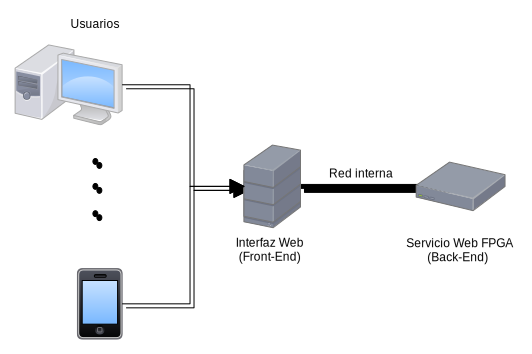
\includegraphics[width=0.7\textwidth,clip=true]{arquitectura}
  \caption{Arquitectura general de la aplicación.}
  \label{fig:arquitectura}
\end{figure}


\section{Back-End - Servicio Web FPGA\label{sec:dis:servicio_web_fpga}}

El componente \gls{back-end} se encarga de la interacción con la sonda de red (implementada en una \gls{FPGA}) y con el resto de partes involucradas en la reproducción y captura de tráfico de red.
Para ello, recibe peticiones \gls{HTTP} del \gls{front-end} (actuando en este caso como cliente), que se traducen en acciones sobre el sistema o en respuestas sobre el estado del mismo.
\begin{figure}[!htp]
  \centering
  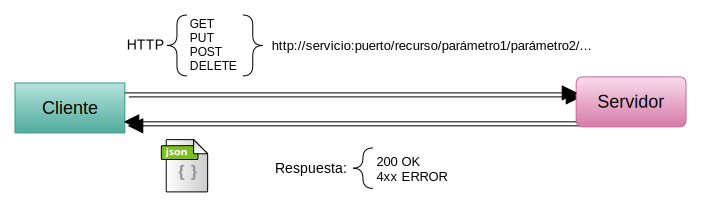
\includegraphics[width=0.95\textwidth,clip=true]{fpga_rest}
  \caption{Diagrama de flujo de un servicio \gls{REST}.}
  \label{fig:fpga_rest}
\end{figure}

La arquitectura de comunicación externa del \gls{back-end} se basa en el modelo de cliente-servidor \gls{REST} (ver Figura \ref{fig:fpga_rest}). Dentro de las directrices que marca este modelo, sólo se han considerado útiles para el problema dado un subconjunto de ellas:
\begin{itemize}
  \item El protocolo entre el cliente y el servidor debe ser sin estado: cada mensaje \gls{HTTP} tiene que contener toda la información necesaria para comprender la petición.
  \item Las operciones se aplican sobre recursos mediante llamadas a métodos \gls{HTTP}: \textit{GET} para obtener información sobre un recurso, \textit{POST}/\textit{PUT} para actualizarlos o crearlos y \textit{DELETE} para borrarlos.
  \item Cada recurso debe tener un identificador único (en este caso, una \gls{URL} única).
\end{itemize}

Se ha decidido no adoptar el resto de directrices \gls{REST} debido a que no encajaban dentro del modelo de funcionamiento de la aplicación.
Así, no se facilita el descubrimiento automático de recursos y métodos, ya que se ha considerado que no tiene sentido siendo éste un subsistema interno y no un componente público.
Por otra parte, no se permiten distintas representaciones de un mismo recurso, siendo \gls{JSON} la única representación utilizada.
No seguir estas directrices simplifica además la implementación del \gls{back-end}.

\begin{figure}[!htp]
  \centering
  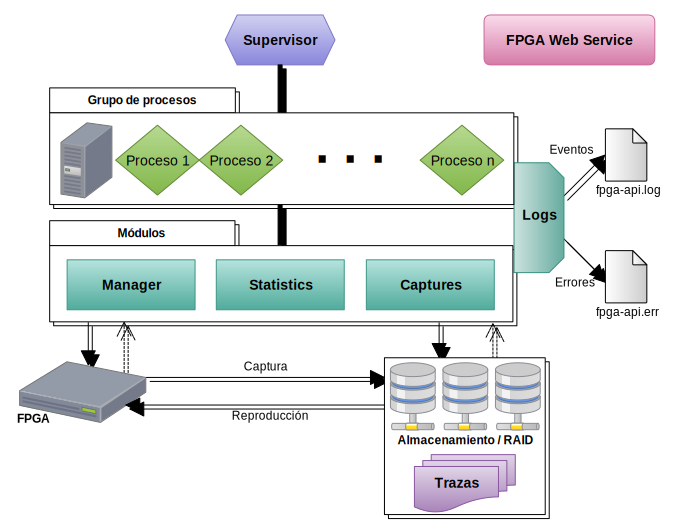
\includegraphics[width=0.95\textwidth,clip=true]{fpga}
  \caption{Arquitectura del \gls{servicioweb} \gls{FPGA}.}
  \label{fig:arquitectura_servicio}
\end{figure}

Internamente, \ref{fig:arquitectura_servicio}, 
Supervisor
1 párrafo Cluster de procesos para operaciones auxiliares, alta disponibilidad \ref{fig:arquitectura_servicio}
Logs
Módulos
Se distinguen por tanto, según su funcionalidad, tres módulos dentro del servicio web: gestión, captura y estadísticas.
\subsection{Gestión\label{ssec:dis:gestion}}

Este módulo tiene dos funciones principales: gestionar el estado de la sonda de red y gese encarga tanto de gestionar el estado de la sonda .
TODO: Gestión
  {Capturador,Reproductor}


\subsection{Capturas\label{ssec:dis:capturas}}

El módulo de capturas se encarga de todos los aspectos relacionados con las \glspl{traza} de tráfico de red.


detectar el formato interno de una \gls{traza}.

TODO: Capturas
  {Detección,Conversión,Renombrado,Borrado}


\subsection{Estadísticas\label{ssec:dis:estadisticas}}

estado, get
TODO: Estado/Estadísticas
  {Velocidad,Estado,RAID}


\section{Front-End - Interfaz web\label{sec:dis:interfaz_web}}

TODO: [Introducción] > sobre el framework, comunicación con el backend

Diseño responsive, visualmente atractiv. ventajas y diferencias vs adaptativo

Internacionalización

Introducción maquetas de las páginas principales

\subsection{Maquetas\label{ssec:dis:maquetas}}

\begin{figure}[!htp]
  \centering
  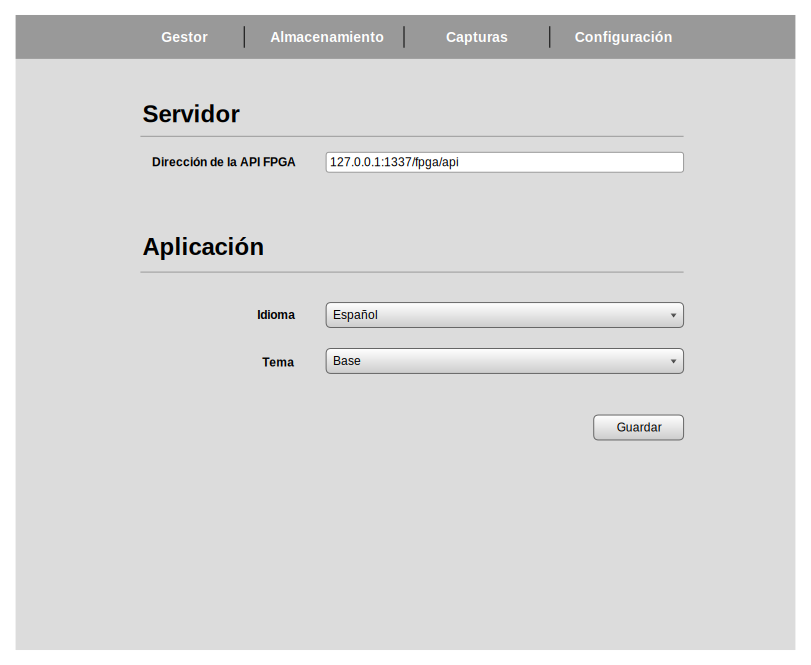
\includegraphics[width=0.95\textwidth,clip=true]{maquetas/maqueta_configuracion}
  \caption{Maqueta de la pantalla de configuración de la aplicación.}
  \label{fig:maqueta:configuracion}
\end{figure}

\begin{figure}[!htp]
  \centering
  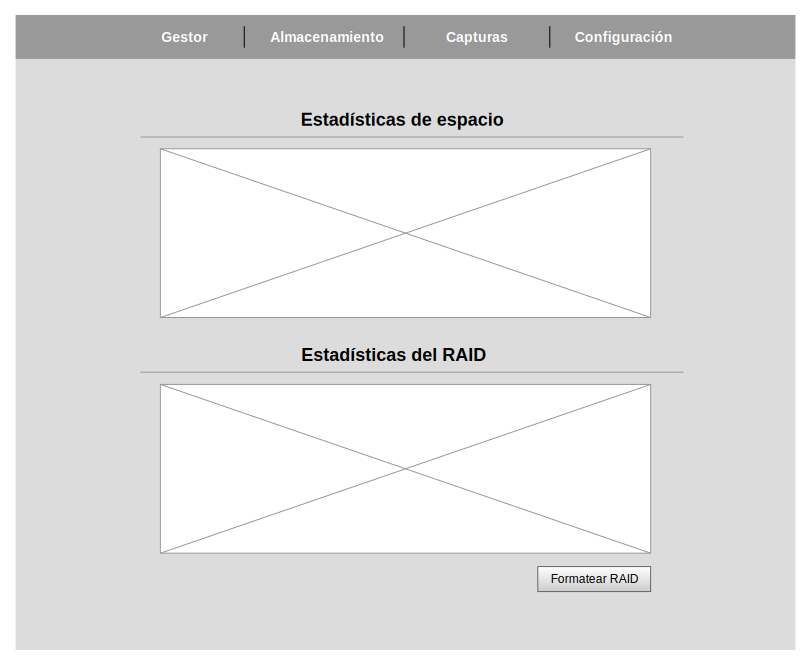
\includegraphics[width=0.95\textwidth,clip=true]{maquetas/maqueta_almacenamiento}
  \caption{Maqueta de la pantalla de almacenamiento.}
  \label{fig:maqueta:almacenamiento}
\end{figure}

\begin{figure}[!htp]
  \centering
  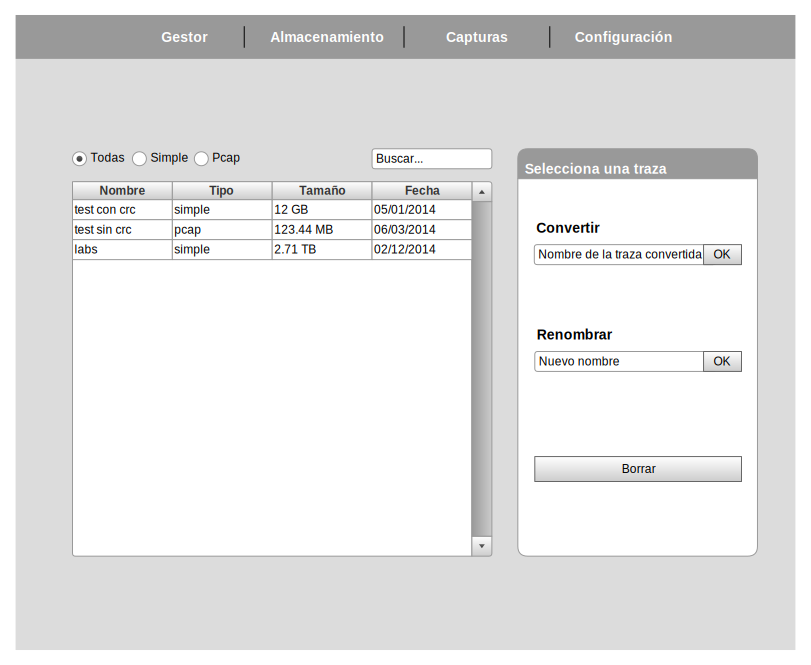
\includegraphics[width=0.95\textwidth,clip=true]{maquetas/maqueta_capturas}
  \caption{Maqueta de la pantalla de gestión de \glspl{traza}.}
  \label{fig:maqueta:capturas}
\end{figure}

\begin{figure}[!htp]
  \centering
  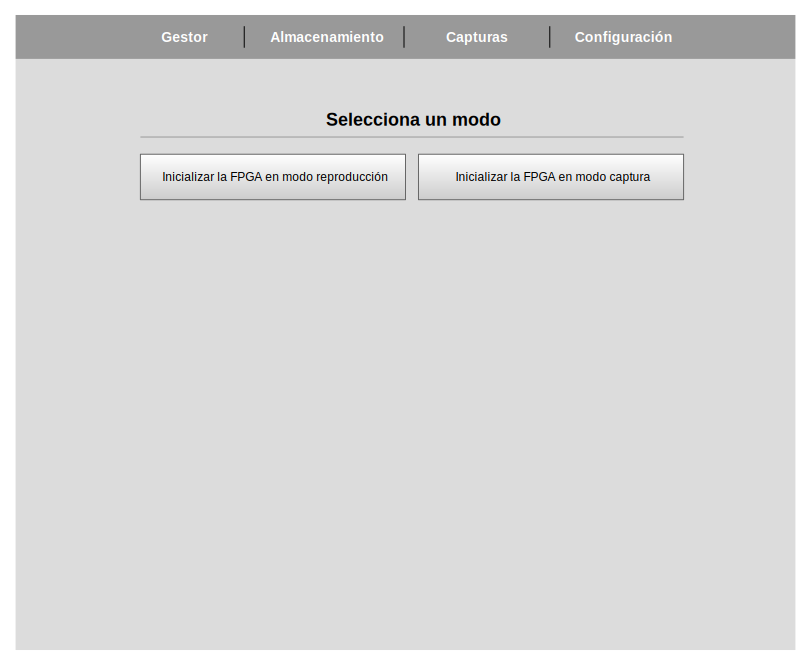
\includegraphics[width=0.95\textwidth,clip=true]{maquetas/maqueta_gestor_seleccion}
  \caption{Maqueta de la pantalla de gestión - selección de modo.}
  \label{fig:maqueta:gestor_seleccion}
\end{figure}

\begin{figure}[!htp]
  \centering
  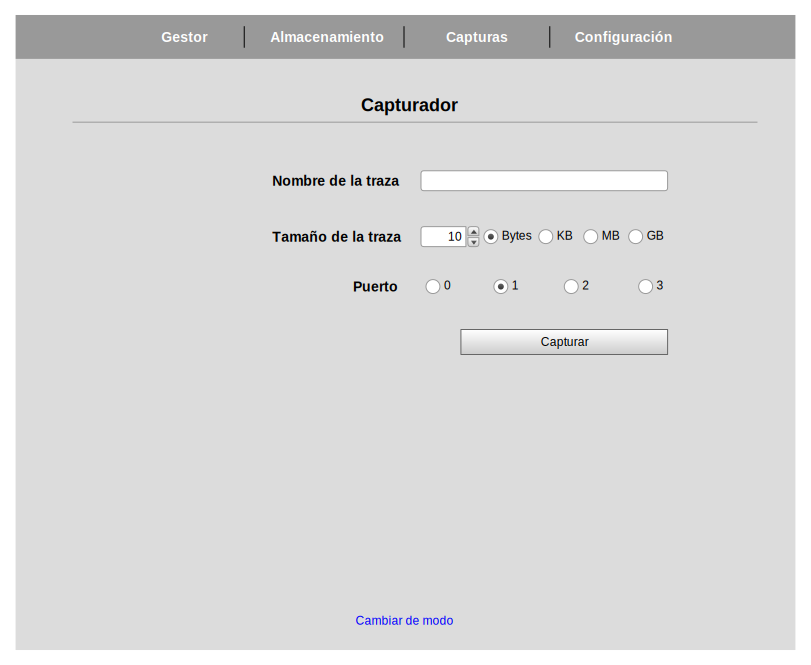
\includegraphics[width=0.95\textwidth,clip=true]{maquetas/maqueta_gestor_capturador}
  \caption{Maqueta de la pantalla de gestión - formulario para capturar.}
  \label{fig:maqueta:gestor_capturador}
\end{figure}

\begin{figure}[!htp]
  \centering
  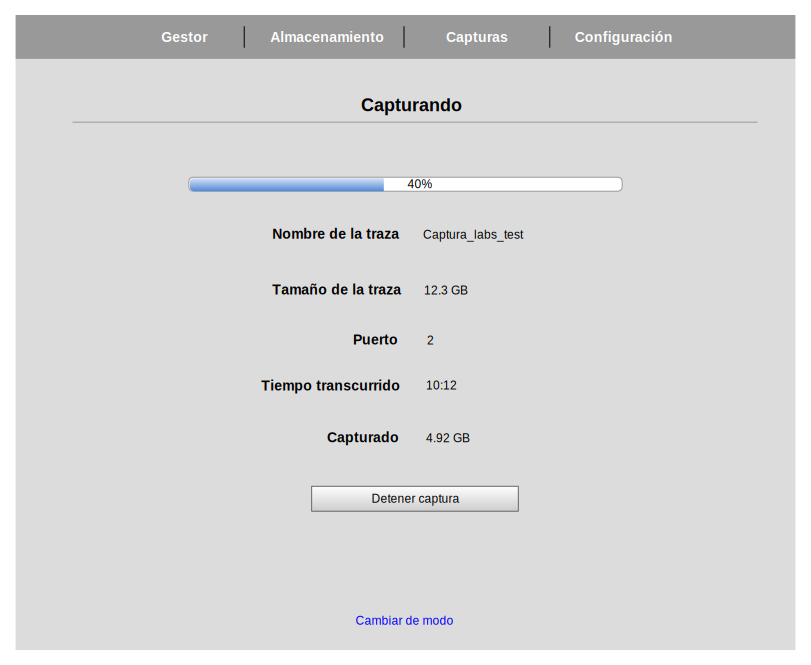
\includegraphics[width=0.95\textwidth,clip=true]{maquetas/maqueta_gestor_capturando}
  \caption{Maqueta de la pantalla de gestión - capturando.}
  \label{fig:maqueta:gestor_capturando}
\end{figure}

\begin{figure}[!htp]
  \centering
  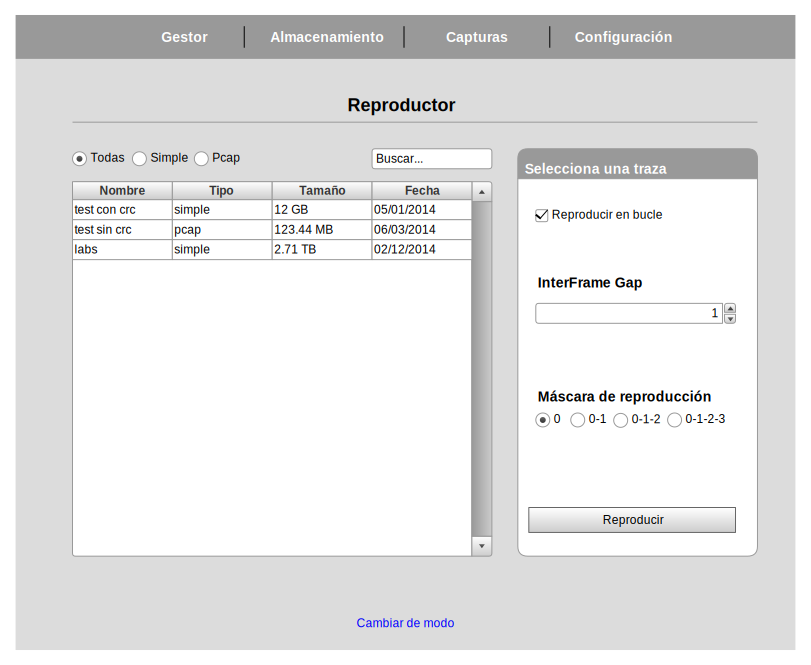
\includegraphics[width=\textwidth,clip=true]{maquetas/maqueta_gestor_reproductor}
  \caption{Maqueta de la pantalla de gestión - formulario para reproducir.}
  \label{fig:maqueta:gestor_reproductor}
\end{figure}

\begin{figure}[!htp]
  \centering
  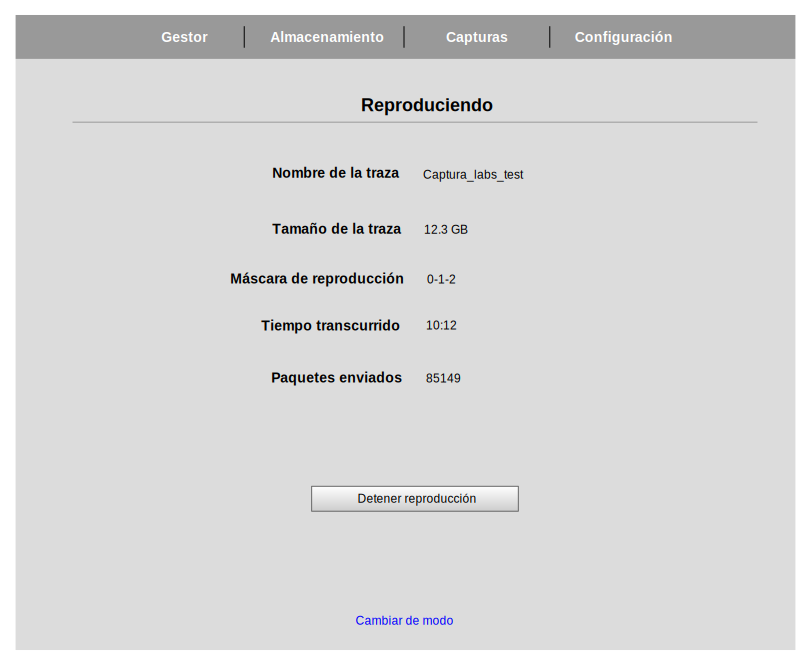
\includegraphics[width=\textwidth,clip=true]{maquetas/maqueta_gestor_reproduciendo}
  \caption{Maqueta de la pantalla de gestión - reproduciendo.}
  \label{fig:maqueta:gestor_reproduciendo}
\end{figure}
\chapter{Implementación\label{cap:implementacion}}

TODO: [Introducción]


\section{Back-End\label{sec:imp:back_end}}

TODO: Back-End
  [Introducción]
  Captura árbol de archivos
  árbol rutas?
  {io.js,express,supervisor,apiDoc,npm}
  {API ~REST,mensajes json}
  {Servicio}


\section{Front-End\label{sec:imp:front_end}}

TODO: Front-End
  [Introducción]
  Capturas diseño responsive
  Capturas árbol de archivos
  - {MVC propio,Bootstrap,jQuery,gettext,phpDocumentor}


\subsection{Internacionalización\label{ssec:imp:internacionalizacion}}

TODO: Localización


\subsection{Temas\label{ssec:imp:temas}}

TODO: Temas
\chapter{Pruebas\label{cap:pruebas}}

TODO: [Introducción]


\section{Pruebas de verificación\label{sec:pb:verificacion}}

TODO: Pruebas de verificación


\section{Pruebas de validación\label{sec:pb:validacion}}

TODO: Pruebas de validación
\chapter{Mantenimiento\label{cap:mantenimiento}}

TODO: [Introducción]
  {Open Source/GitHub Issues/Pull Requests}
\chapter{Conclusiones\label{cap:conclusiones}}

TODO: Conclusiones sobre el trabajo realizado
\include{src/lineasDeTrabajoFuturo}

%
% Página en blanco
%
\cleardoublepage

%
% Bibliografía
%
\bibliography{src/bibliografia}
\addcontentsline{toc}{chapter}{Bibliografía}

%
% Apéndices
%
\appendix
\cleardoublepage
\addappheadtotoc
\appendixpage

% No expandir elementos para llenar toda la página
\raggedbottom

%
% Apéndices del TFG
%
\chapter{Manual de Usuario\label{extra:manual_de_usuario}}

Este manual pretende ser una guía en la instalación, configuración y uso de la interfaz web para la gestión de sondas de red de altas prestaciones.

\section{Instalación del Servicio Web FPGA\label{extra:manual:instalacionfpga}}

\subsection*{Requisitos}
El servidor que aloje el \gls{servicioweb} \gls{FPGA} debe cumplir los siguientes requisitos:
\begin{itemize}
  \item La \gls{FPGA} para capturar/reproducir tráfico debe estar conectada.
  \item El sistema operativo debe estar basado en una distribución \textit{Debian} \cite{debian} y tener una arquitectura de 64 bits.
  \item La opción por defecto en el gestor de arranque debe ser iniciar con la opción \textit{HugePages} activa.
  \item El usuario \textit{root} debe existir.
\end{itemize}

\subsection*{Instalación}
Para instalar el \gls{servicioweb} \gls{FPGA}, compruebe que se cumplan todos los requisitos y siga los siguientes pasos:
\begin{enumerate}
  \item Descargue el código fuente del repositorio del proyecto (\href{https://github.com/JSidrach/NetWatcher/archive/master.zip}{\footnotesize{github.com/JSidrach/NetWatcher}}). La instalación se realiza de forma remota, así que no es necesario descargárselo en el propio servidor, aunque sí en un entorno con terminal.
  \item Descomprima el archivo \textit{.zip}.
  \item Edite el archivo \texttt{./fpga-api/scripts/update\_server.sh}, estableciendo los parámetros \texttt{SERVER\_IP} y \texttt{SERVER\_PATH} como la dirección del servidor remoto que alojará el \gls{servicioweb} \gls{FPGA} y la ruta donde guardar el código, respectivamente.
  \item Sitúese en la carpeta \texttt{./fpga-api/}.
  \item Despliegue el servidor ejecutando el siguiente comando:
  
  \texttt{./scripts/update\_server.sh}.
  \item Inicie sesión en el servidor remoto.
  \item Ponga en marcha el \gls{servicioweb} ejecutando el siguiente comando:

  \texttt{sudo service fpga-api start}
  \item Compruebe que el servidor está activo con el siguiente comando:

  \texttt{sudo service fpga-api status}
\end{enumerate}


\section{Configuración del Servicio Web FPGA\label{extra:manual:configfpga}}
Para configurar el \gls{servicioweb} \gls{FPGA}, inicie sesión en el servidor en el que se instaló este servicio. Los distintos parámetros de configuración vienen recogidos en el archivo \texttt{config.js}, dentro de la carpeta raíz del servicio (el contenido de la variable \texttt{SERVER\_PATH}, establecida en la instalación). Edite las distintas variables de este archivo (explicadas en la Tabla \ref{extra:manual:paramsfpga}) para configurar el servicio. No es necesario reiniciar el servicio para que los cambios en el archivo \texttt{config.js} se reflejen en el servidor.

\begin{table}
\centering
\begin{tabular}{|l|l|l|}
\hline
\rowcolor[HTML]{F5F5F5}
\textbf{Variable}   & \textbf{Tipo}    & \textbf{Descripción}                                           \\ \hline
BASE\_PREFIX        & Cadena de texto  & Prefijo base de la \gls{API}                                   \\ \hline
PORT                & Número entero    & Puerto del servicio                                            \\ \hline
MAX\_DELAY          & Número entero    & Retraso máximo entre el \textit{timestamp} de las              \\
                    &                  & peticiones y el \textit{timestamp} del servidor. Si            \\
                    &                  & es menor o igual que 0, no se descartará                       \\ 
                    &                  & ninguna petición basándose en el \textit{timestamp}            \\ \hline
IMPACT\_BIN         & Cadena de texto  & Ruta al ejecutable \texttt{impact} de \textit{Xilinx}          \\ \hline
CAPTURES\_DIR       & Cadena de texto  & Directorio donde se guardarán las \glspl{traza}                \\
                    &                  & (debe acabar en /)                                             \\ \hline
RAID                & Booleano         & Bandera que indica si el \gls{RAID} está activo o              \\
                    &                  & o no. Establezca esta variable como \textit{true}              \\
                    &                  & sólo si \texttt{CAPTURES\_DIR} está sobre un \gls{RAID} y      \\
                    &                  & las variables \texttt{RAID\_DEV} y \texttt{RAID\_DISKS} están  \\
                    &                  & asignadas.                                                     \\ \hline
RAID\_DEV           & Cadena de texto  & Ruta al \gls{RAID}                                             \\ \hline
RAID\_DISKS         & Array de cadenas & Discos físicos del \gls{RAID} (por ejemplo:                    \\
                    &                  & \texttt{/dev/sdc}, \texttt{/dev/sdd}, etc.)                    \\ \hline
\end{tabular}
\caption{Variables de configuración del \gls{servicioweb} \gls{FPGA}}
\label{extra:manual:paramsfpga}
\end{table}

\section{Instalación de la interfaz web\label{extra:manual:instalacionweb}}

\subsection*{Requisitos}
El servidor que aloje la interfaz web debe cumplir los siguientes requisitos:
\begin{itemize}
  \item \textit{Apache httpd} \cite{httpd} debe estar instalado.
  \item La dirección del \gls{servicioweb} \gls{FPGA} debe ser accesible desde este servidor.
\end{itemize}

\subsection*{Instalación}
Para instalar la interfaz web, compruebe que se cumplan todos los requisitos y siga los siguientes pasos:
\begin{enumerate}
  \item Descargue el código fuente del repositorio del proyecto (\href{https://github.com/JSidrach/NetWatcher/archive/master.zip}{\footnotesize{github.com/JSidrach/NetWatcher}}).
  \item Descomprima el \textit{.zip} y mueva la carpeta base \textit{NetWatcher} al directorio público de \textit{Apache} (normalmente \texttt{/var/www/html/}).
  \item Sitúese en la carpeta base \textit{NetWatcher}.
  \item Instale los paquetes y librerías necesarios ejecutando el siguiente comando:

  \texttt{sudo ./scripts/build.sh --install}
\end{enumerate}


\section{Configuración de la interfaz web\label{extra:manual:configweb}}
TODO: Configuración - IP, tema, idioma


\section{Uso de la aplicación\label{extra:manual:uso}}
Una vez instalado y configurado tanto el \gls{servicioweb} \gls{FPGA} como la interfaz web.
TODO: [Introducción]. Rutas arriba, rutas abajo, documentaciones


\section{Solución de problemas\label{extra:manual:solucion}}

Si tras seguir las instrucciones paso a paso algo impide el correcto funcionamiento de la aplicación, puedes consultar la página de solución de problemas (en inglés), disponible dentro del repositorio del proyecto en:

\href{https://github.com/JSidrach/NetWatcher/blob/master/docs/wiki/Troubleshooting.md}{github.com/JSidrach/NetWatcher/blob/master/docs/wiki/Troubleshooting.md}
\include{src/frameworkDesarrollado}
\include{src/apiServicioWebFpga}

% Fin del documento
\end{document}